\documentclass{standalone}
\usepackage{tikz}
\usetikzlibrary{patterns, positioning}


\begin{document}
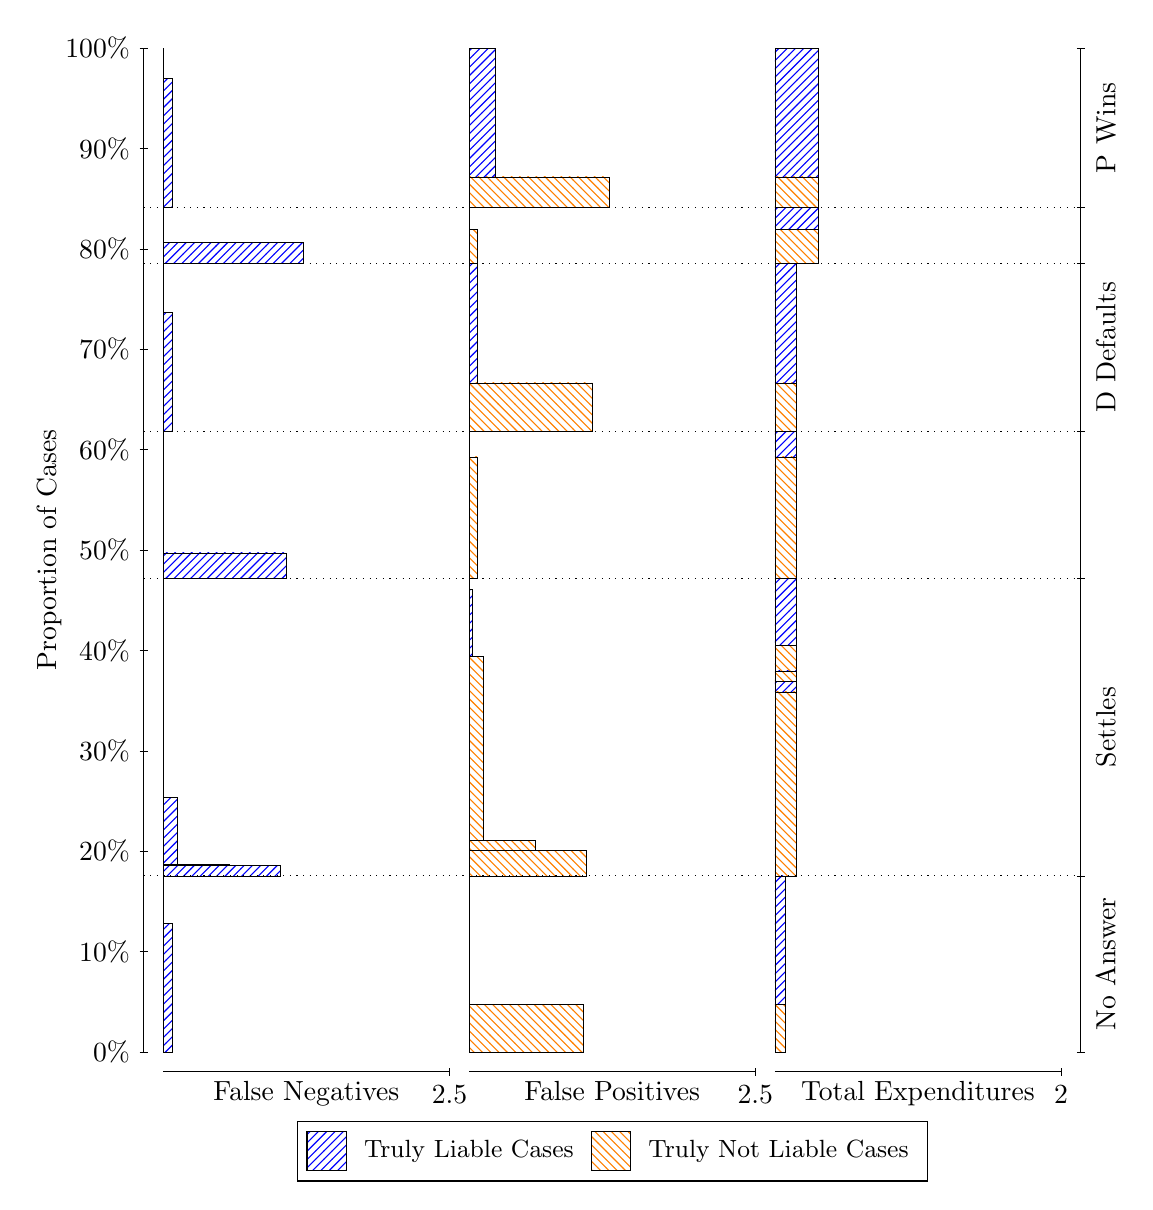
\begin{tikzpicture}
\draw[black, very thin] (1.5,1.75) -- (1.5,14.5);
\node[rotate=90, text=black, anchor=center] at (0.3, 8.125) {Proportion of Cases};
\draw[black, very thin] (1.45,1.75) -- (1.55,1.75);
\node[text=black, anchor=east] at (1.45, 1.75) {0\%};
\draw[black, very thin] (1.45,3.025) -- (1.55,3.025);
\node[text=black, anchor=east] at (1.45, 3.025) {10\%};
\draw[black, very thin] (1.45,4.3) -- (1.55,4.3);
\node[text=black, anchor=east] at (1.45, 4.3) {20\%};
\draw[black, very thin] (1.45,5.575) -- (1.55,5.575);
\node[text=black, anchor=east] at (1.45, 5.575) {30\%};
\draw[black, very thin] (1.45,6.85) -- (1.55,6.85);
\node[text=black, anchor=east] at (1.45, 6.85) {40\%};
\draw[black, very thin] (1.45,8.125) -- (1.55,8.125);
\node[text=black, anchor=east] at (1.45, 8.125) {50\%};
\draw[black, very thin] (1.45,9.4) -- (1.55,9.4);
\node[text=black, anchor=east] at (1.45, 9.4) {60\%};
\draw[black, very thin] (1.45,10.675) -- (1.55,10.675);
\node[text=black, anchor=east] at (1.45, 10.675) {70\%};
\draw[black, very thin] (1.45,11.95) -- (1.55,11.95);
\node[text=black, anchor=east] at (1.45, 11.95) {80\%};
\draw[black, very thin] (1.45,13.225) -- (1.55,13.225);
\node[text=black, anchor=east] at (1.45, 13.225) {90\%};
\draw[black, very thin] (1.45,14.5) -- (1.55,14.5);
\node[text=black, anchor=east] at (1.45, 14.5) {100\%};

\draw[black, very thin] (13.4,1.75) -- (13.4,14.5);
\draw[black, very thin] (13.35,1.75) -- (13.45,1.75);
\node[anchor=west] at (13.35, 1.75) {};
\draw[black, very thin] (13.35,3.9877) -- (13.45,3.9877);
\node[anchor=west] at (13.35, 3.9877) {};
\draw[black, very thin] (13.35,7.7663) -- (13.45,7.7663);
\node[anchor=west] at (13.35, 7.7663) {};
\draw[black, very thin] (13.35,9.6309) -- (13.45,9.6309);
\node[anchor=west] at (13.35, 9.6309) {};
\draw[black, very thin] (13.35,11.762) -- (13.45,11.762);
\node[anchor=west] at (13.35, 11.762) {};
\draw[black, very thin] (13.35,12.474) -- (13.45,12.474);
\node[anchor=west] at (13.35, 12.474) {};
\draw[black, very thin] (13.35,14.5) -- (13.45,14.5);
\node[anchor=west] at (13.35, 14.5) {};

\draw[black, very thin, pattern color=blue, pattern=north east lines] (1.75,1.75) rectangle (1.859,3.3838);
\draw[black, very thin, pattern color=orange, pattern=north west lines] (1.75,3.3838) rectangle (1.75,3.9877);
\draw[black, very thin, pattern color=blue, pattern=north east lines] (1.75,3.9877) rectangle (3.2397,4.1205);
\draw[black, very thin, pattern color=blue, pattern=north east lines] (1.75,4.1205) rectangle (2.5857,4.1292);
\draw[black, very thin, pattern color=blue, pattern=north east lines] (1.75,4.1292) rectangle (1.9317,4.9788);
\draw[black, very thin, pattern color=orange, pattern=north west lines] (1.75,4.9788) rectangle (1.75,7.7663);
\draw[black, very thin, pattern color=blue, pattern=north east lines] (1.75,7.7663) rectangle (3.3123,8.0894);
\draw[black, very thin, pattern color=orange, pattern=north west lines] (1.75,8.0894) rectangle (1.75,9.6309);
\draw[black, very thin, pattern color=blue, pattern=north east lines] (1.75,9.6309) rectangle (1.859,11.147);
\draw[black, very thin, pattern color=orange, pattern=north west lines] (1.75,11.147) rectangle (1.75,11.762);
\draw[black, very thin, pattern color=blue, pattern=north east lines] (1.75,11.762) rectangle (3.5303,12.035);
\draw[black, very thin, pattern color=orange, pattern=north west lines] (1.75,12.035) rectangle (1.75,12.474);
\draw[black, very thin, pattern color=blue, pattern=north east lines] (1.75,12.474) rectangle (1.859,14.111);
\draw[black, very thin, pattern color=orange, pattern=north west lines] (1.75,14.111) rectangle (1.75,14.5);
\draw[black, very thin, pattern color=orange, pattern=north west lines] (5.6333,1.75) rectangle (7.0867,2.3539);
\draw[black, very thin, pattern color=blue, pattern=north east lines] (5.6333,2.3539) rectangle (5.6333,3.9877);
\draw[black, very thin, pattern color=orange, pattern=north west lines] (5.6333,3.9877) rectangle (7.123,4.3141);
\draw[black, very thin, pattern color=orange, pattern=north west lines] (5.6333,4.3141) rectangle (6.469,4.4396);
\draw[black, very thin, pattern color=orange, pattern=north west lines] (5.6333,4.4396) rectangle (5.815,6.7752);
\draw[black, very thin, pattern color=blue, pattern=north east lines] (5.6333,6.7752) rectangle (5.6697,7.6248);
\draw[black, very thin, pattern color=blue, pattern=north east lines] (5.6333,7.6248) rectangle (5.6333,7.7663);
\draw[black, very thin, pattern color=orange, pattern=north west lines] (5.6333,7.7663) rectangle (5.7423,9.3078);
\draw[black, very thin, pattern color=blue, pattern=north east lines] (5.6333,9.3078) rectangle (5.6333,9.6309);
\draw[black, very thin, pattern color=orange, pattern=north west lines] (5.6333,9.6309) rectangle (7.1957,10.246);
\draw[black, very thin, pattern color=blue, pattern=north east lines] (5.6333,10.246) rectangle (5.7423,11.762);
\draw[black, very thin, pattern color=orange, pattern=north west lines] (5.6333,11.762) rectangle (5.7423,12.201);
\draw[black, very thin, pattern color=blue, pattern=north east lines] (5.6333,12.201) rectangle (5.6333,12.474);
\draw[black, very thin, pattern color=orange, pattern=north west lines] (5.6333,12.474) rectangle (7.4137,12.863);
\draw[black, very thin, pattern color=blue, pattern=north east lines] (5.6333,12.863) rectangle (5.9603,14.5);
\draw[black, very thin, pattern color=orange, pattern=north west lines] (9.5167,1.75) rectangle (9.6529,2.3539);
\draw[black, very thin, pattern color=blue, pattern=north east lines] (9.5167,2.3539) rectangle (9.6529,3.9877);
\draw[black, very thin, pattern color=orange, pattern=north west lines] (9.5167,3.9877) rectangle (9.7892,6.3234);
\draw[black, very thin, pattern color=blue, pattern=north east lines] (9.5167,6.3234) rectangle (9.7892,6.4562);
\draw[black, very thin, pattern color=orange, pattern=north west lines] (9.5167,6.4562) rectangle (9.7892,6.5816);
\draw[black, very thin, pattern color=blue, pattern=north east lines] (9.5167,6.5816) rectangle (9.7892,6.5903);
\draw[black, very thin, pattern color=orange, pattern=north west lines] (9.5167,6.5903) rectangle (9.7892,6.9167);
\draw[black, very thin, pattern color=blue, pattern=north east lines] (9.5167,6.9167) rectangle (9.7892,7.7663);
\draw[black, very thin, pattern color=orange, pattern=north west lines] (9.5167,7.7663) rectangle (9.7892,9.3078);
\draw[black, very thin, pattern color=blue, pattern=north east lines] (9.5167,9.3078) rectangle (9.7892,9.6309);
\draw[black, very thin, pattern color=orange, pattern=north west lines] (9.5167,9.6309) rectangle (9.7892,10.246);
\draw[black, very thin, pattern color=blue, pattern=north east lines] (9.5167,10.246) rectangle (9.7892,11.762);
\draw[black, very thin, pattern color=orange, pattern=north west lines] (9.5167,11.762) rectangle (10.062,12.201);
\draw[black, very thin, pattern color=blue, pattern=north east lines] (9.5167,12.201) rectangle (10.062,12.474);
\draw[black, very thin, pattern color=orange, pattern=north west lines] (9.5167,12.474) rectangle (10.062,12.863);
\draw[black, very thin, pattern color=blue, pattern=north east lines] (9.5167,12.863) rectangle (10.062,14.5);
\draw[black, dotted] (1.5,3.9877) -- (13.4,3.9877);
\draw[black, dotted] (1.5,7.7663) -- (13.4,7.7663);
\draw[black, dotted] (1.5,9.6309) -- (13.4,9.6309);
\draw[black, dotted] (1.5,11.762) -- (13.4,11.762);
\draw[black, dotted] (1.5,12.474) -- (13.4,12.474);
\draw[black, very thin] (1.75,1.5) -- (5.3833,1.5);
\node[text=black, anchor=north] at (3.5667, 1.5) {False Negatives};
\draw[black, very thin] (5.3833,1.45) -- (5.3833,1.55);
\node[text=black, anchor=north] at (5.3833, 1.45) {2.5};

\draw[black, very thin] (5.6333,1.5) -- (9.2667,1.5);
\node[text=black, anchor=north] at (7.45, 1.5) {False Positives};
\draw[black, very thin] (9.2667,1.45) -- (9.2667,1.55);
\node[text=black, anchor=north] at (9.2667, 1.45) {2.5};

\draw[black, very thin] (9.5167,1.5) -- (13.15,1.5);
\node[text=black, anchor=north] at (11.333, 1.5) {Total Expenditures};
\draw[black, very thin] (13.15,1.45) -- (13.15,1.55);
\node[text=black, anchor=north] at (13.15, 1.45) {2};

\node[text=black, centered, rotate=90] at (13.72, 2.8689) {No Answer};
\node[text=black, centered, rotate=90] at (13.72, 5.877) {Settles};

\node[text=black, centered, rotate=90] at (13.72, 10.697) {D Defaults};

\node[text=black, centered, rotate=90] at (13.72, 13.487) {P Wins};

\draw (7.449999999999999,1.5) node[draw=none] (baseCoordinate) {};
\begin{scope}[align=center]
        \matrix[scale=0.5, draw=black, below=0.5cm of baseCoordinate, nodes={draw}, column sep=0.1cm]{
            \node[rectangle, draw, minimum width=0.5cm, minimum height=0.5cm, pattern color=blue, pattern=north east lines] {}; &
            \node[draw=none, font=\small, text=black] (B) {Truly Liable Cases}; &
            \node[rectangle, draw, minimum width=0.5cm, minimum height=0.5cm, pattern color=orange, pattern=north west lines] {}; &
            \node[draw=none, font=\small, text=black] (B) {Truly Not Liable Cases}; \\
            };
\end{scope}

\end{tikzpicture}
\end{document}